\chapter{Sampling CT Signals}

Up until now in the course we have focused on either CT or DT signals and systems. Practical systems though often are hybrid and require conversion between DT and CT signals. For example a CT audio signal might be converted to a DT audio signal for storage and/or transmission, and at a later time or location converted back to a CT signal for playback through a speaker.

It is also common to design a CT system and then implement it as a DT system. Advantages of this approach are e.g. such implementations are less susceptible to component variations, require no tuning a build time, are easier to change (firmware or software update), easier to prototype, and more easily use encryption. 

In this lecture we focus on \emph{sampling} of CT signals to produce a DT signal $x[n] = x(nT)$ with sample index $n$ and sample time $T$. In the next lecture we consider the case of converting from a DT to CT signal. 

\section{Sampling Theory}

The process of sampling is to produce a DT signal $x[n]$ from a CT signal $x(t)$ by sampling time at regular intervals $T\in \mathbb{R}^+$ called the \emph{sample-time}, or equivalently sampling at a frequency of $\tfrac{1}{T}$ Hz or $\tfrac{2\pi}{T}$ rad/s. Mathematically this is simple to express in the time domain as $x[n] = x(nT)$, however we seek a system that can perform this task.

Recall the impulse train is the periodic signal
\[
x_1(t) = \sum\limits_{n=-\infty}^{\infty} \delta(t-nT_0)
\]
with period $T_0$ and frequency $\omega_0 = \tfrac{2\pi}{T_0}$. The exponential CT Fourier series of the impulse train is given by
\[
x_1(t) = \sum\limits_{n=-\infty}^{\infty} a_n e^{j\tfrac{2\pi}{T_0}nt}
\]
where the Fourier series coefficients are
\[
a_n = \frac{1}{T_0} \int\limits_{-\frac{T_0}{2}}^{\frac{T_0}{2}} \delta(t) e^{-jn\omega_0 t} \; dt = \frac{1}{T_0} 
\]
Now, lets take the Fourier Transform of the Fourier series representation
\begin{align*}
X_1(j\omega) &= \int\limits_{-\infty}^{\infty} \sum\limits_{n=-\infty}^{\infty} \frac{1}{T_0} e^{j\tfrac{2\pi}{T_0}nt}e^{j\omega t}\; dt\\
&= \frac{1}{T_0} \sum\limits_{n=-\infty}^{\infty} \int\limits_{-\infty}^{\infty} e^{j\tfrac{2\pi}{T_0}nt}e^{j\omega t}\; dt\\
&= \frac{2\pi}{T_0} \sum\limits_{n=-\infty}^{\infty} \delta(\omega - \omega_0 n)
\end{align*}
also an impulse train in the frequency domain. Now suppose we have another signal $x_2(t)$ and we multiply $x_1(t)$ and $x_2(t)$ to get a signal $y(t)$.
\[
y(t) = x_1(t) \cdot x_2(t) = \sum\limits_{n=-\infty}^{\infty} x_2(t) \delta(t-nT_0) = \sum\limits_{n=-\infty}^{\infty} x_2(nT_0) \delta(t-nT_0)
\]
Since $y(t)$ is non-zero only at the locations of the delta functions, we can treat $y(nT_0) = x_2(nT_0)$ as the DT signal $x_2[n]$. This is illustrated below

\begin{center}
  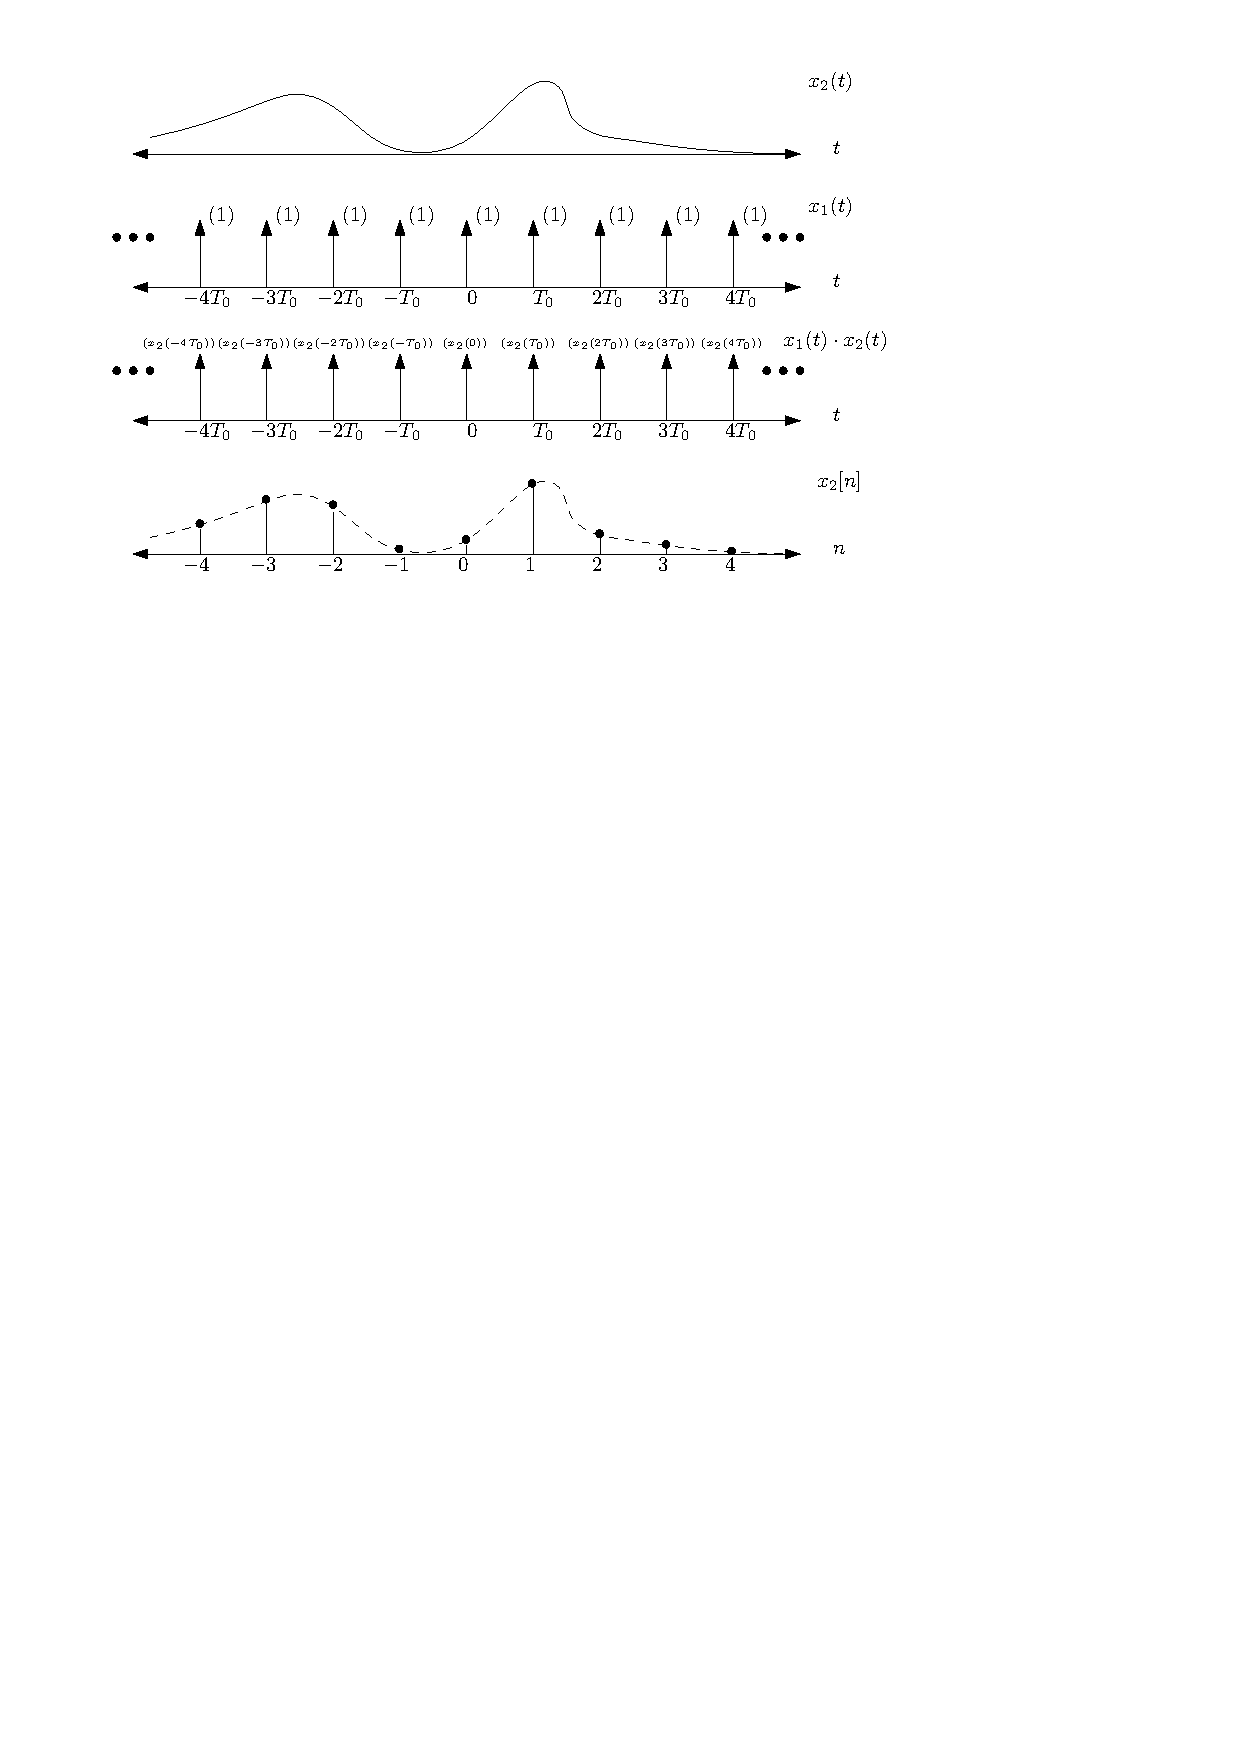
\includegraphics[scale=1]{graphics/samplinf_timedomain.pdf}
\end{center}

Equivalently in the frequency domain the modulation theorem gives
\[
y(t) = x_1(t) \cdot x_2(t) \stackrel{\mathcal{F}}{\longleftrightarrow} \frac{1}{2\pi} X_1(j\omega) * X_2(j\omega) = Y(j\omega)
\]
Lets do the convolution
\begin{align*}
  Y(j\omega) &= \frac{1}{2\pi} X_1(j\omega) * X_2(j\omega)\\
  &=  \frac{1}{2\pi} \left[  \frac{2\pi}{T_0} \sum\limits_{n=-\infty}^{\infty} \delta(\omega - \omega_0 n) \right] * X_2(j\omega)\\
  &= \frac{1}{2\pi} \int\limits_{-\infty}^{\infty}  \frac{2\pi}{T_0} \sum\limits_{n=-\infty}^{\infty} \delta(\omega - \omega^\prime - \omega_0 n) X_2(j\omega^\prime) \; d\omega^\prime\\
  &= \frac{1}{T_0} \sum\limits_{n=-\infty}^{\infty} X_2(j(\omega - n\omega_0)) 
\end{align*}
Thus the sampling process in the frequency domain causes periodic replication of the Fourier transform of the signal being sampled, $x_2(t)$, which are sometimes called \emph{images}. This signal $Y(j\omega)$ is periodic in $\omega_0 = \tfrac{2\pi}{T_0}$ \emph{radians per second} and corresponds to the DT Fourier Transform of $x_2[n]  \stackrel{\mathcal{F}}{\longleftrightarrow} X_2\left(e^{j\omega}\right)$, which is periodic in $2\pi$ \emph{radians per sample time}.

To help us visualize this, suppose that the signal $x_2(t)  \stackrel{\mathcal{F}}{\longleftrightarrow} X_2(j\omega)$ is \emph{band-limited} to $B$ Hz, that is $X_2(j\omega) = 0$ for all frequencies outside the band $-2\pi B < \omega < 2\pi B$. This is shown schematically as the magnitude spectrum below:

\begin{center}
  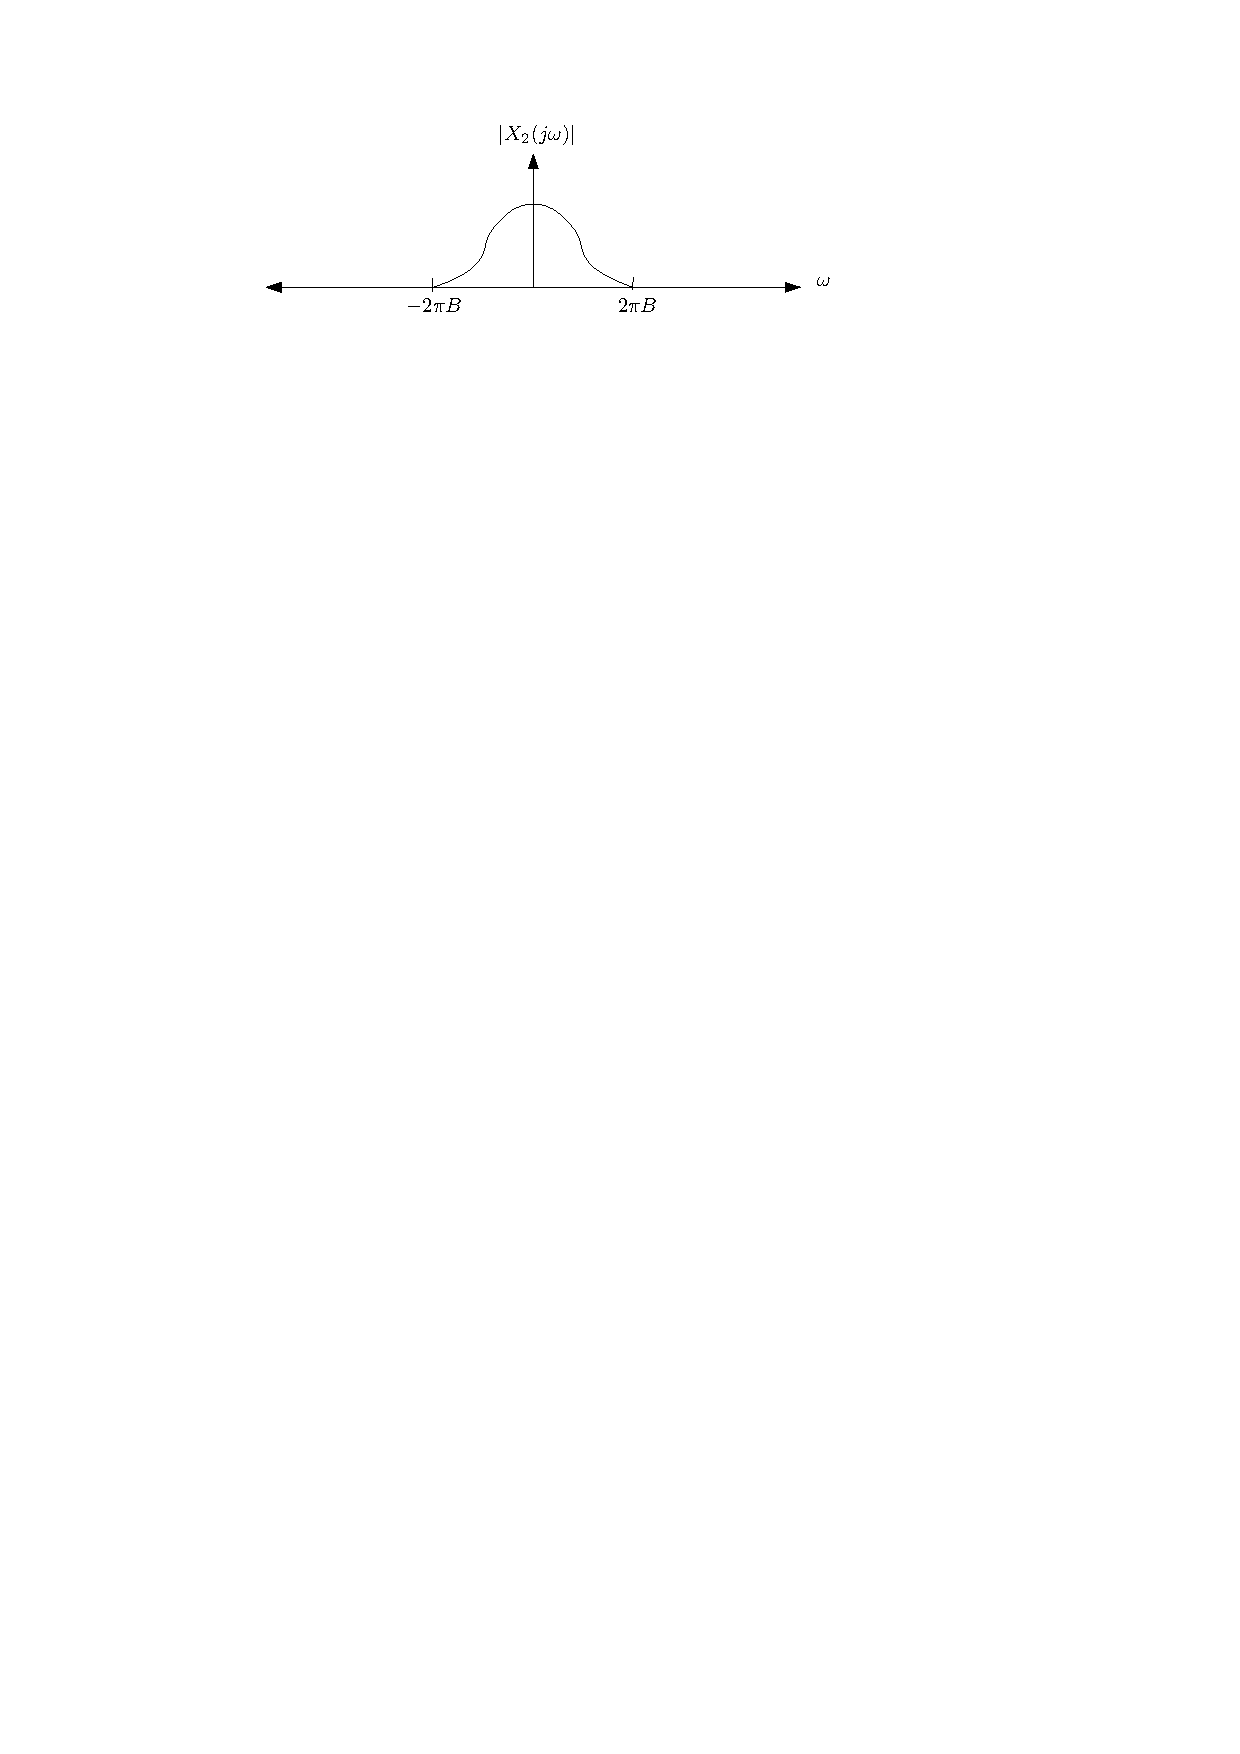
\includegraphics[scale=1]{graphics/bandlimited.pdf}
\end{center}
After sampling ($y(t) = x_1(t)\cdot x_2(t)$) and assuming $\omega_0 > 4\pi B$ the spectrum of the sampled signal is:
\begin{center}
  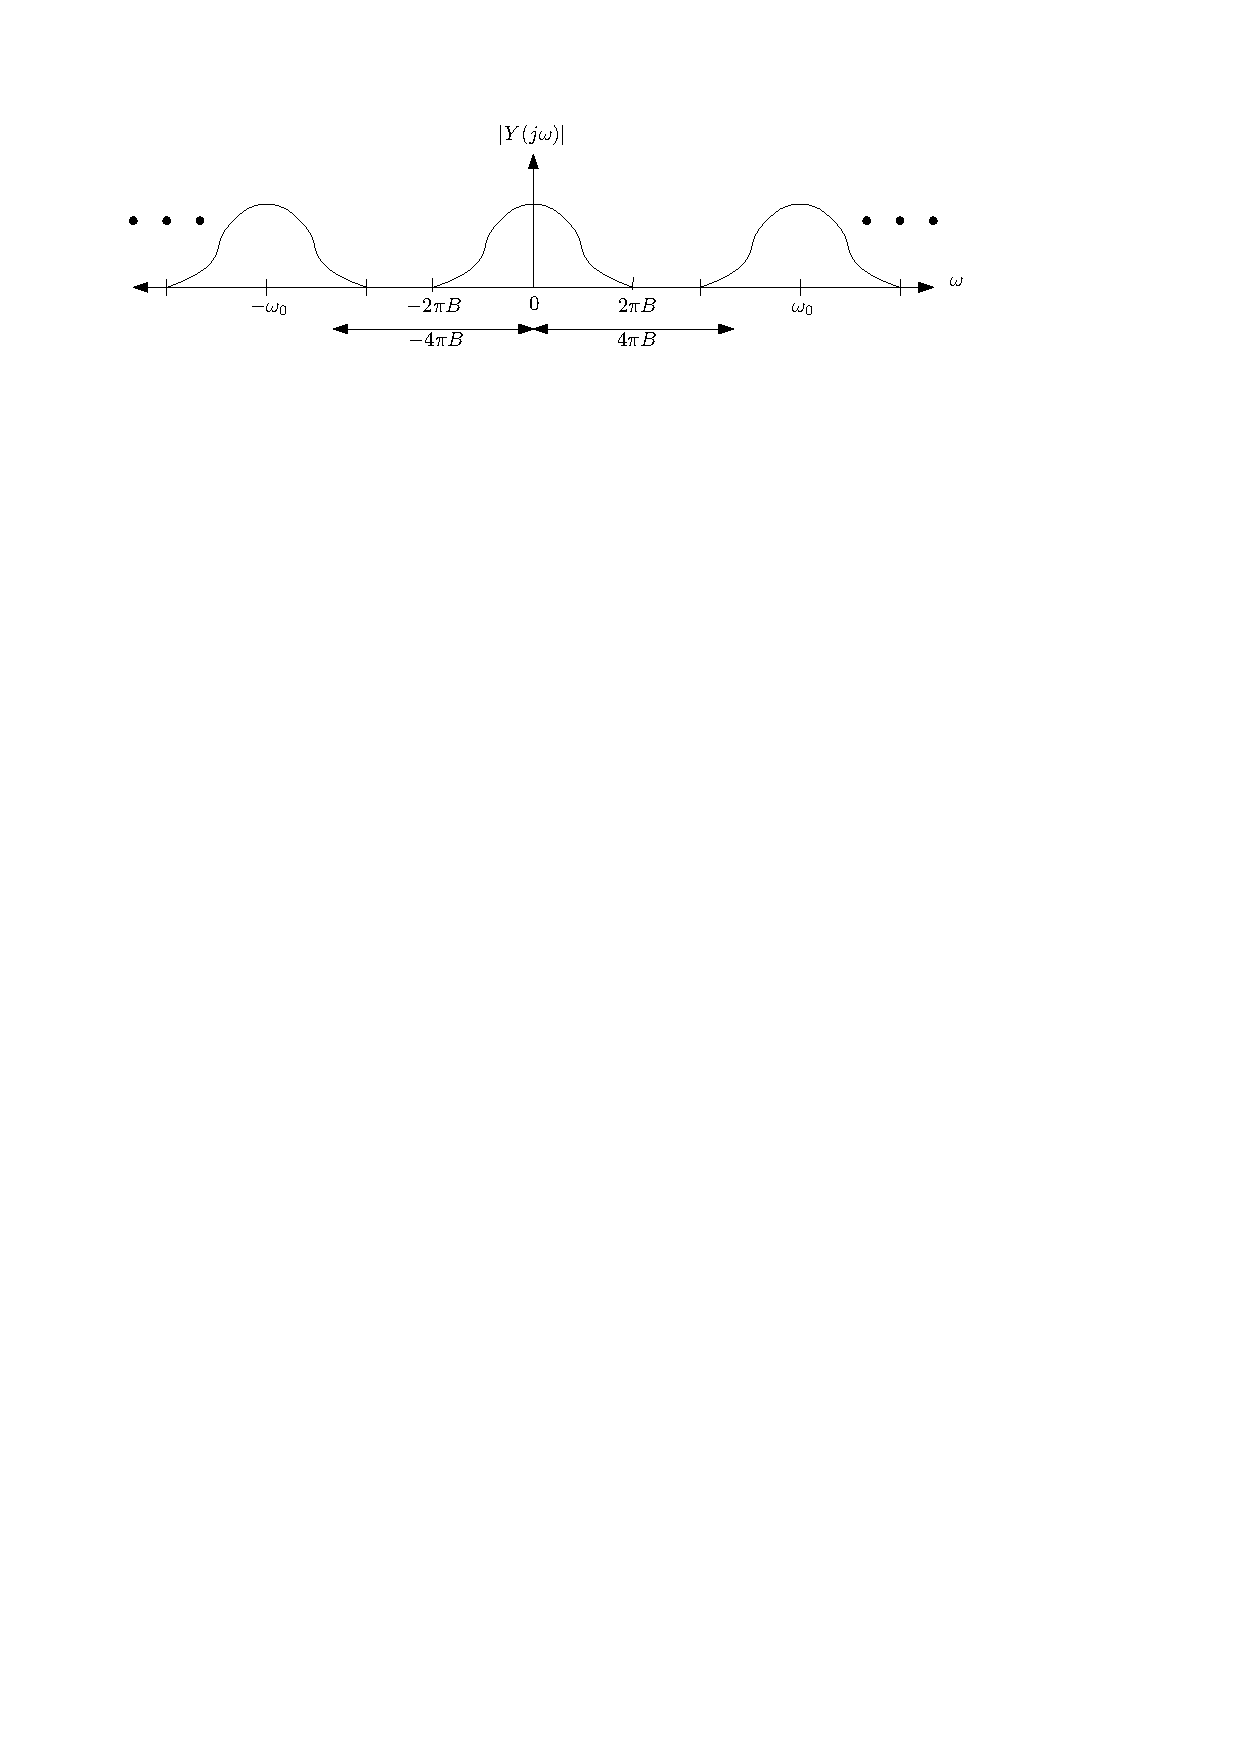
\includegraphics[scale=1]{graphics/bandlimitedsampled1.pdf}
\end{center}
If instead $\omega_0 < 4\pi B$ the images overlap and we get \emph{aliasing}, where high frequency content gets added to the lower frequency content. This is shown below with the lighter lines showing the images and the heavier line showing their sum.
\begin{center}
  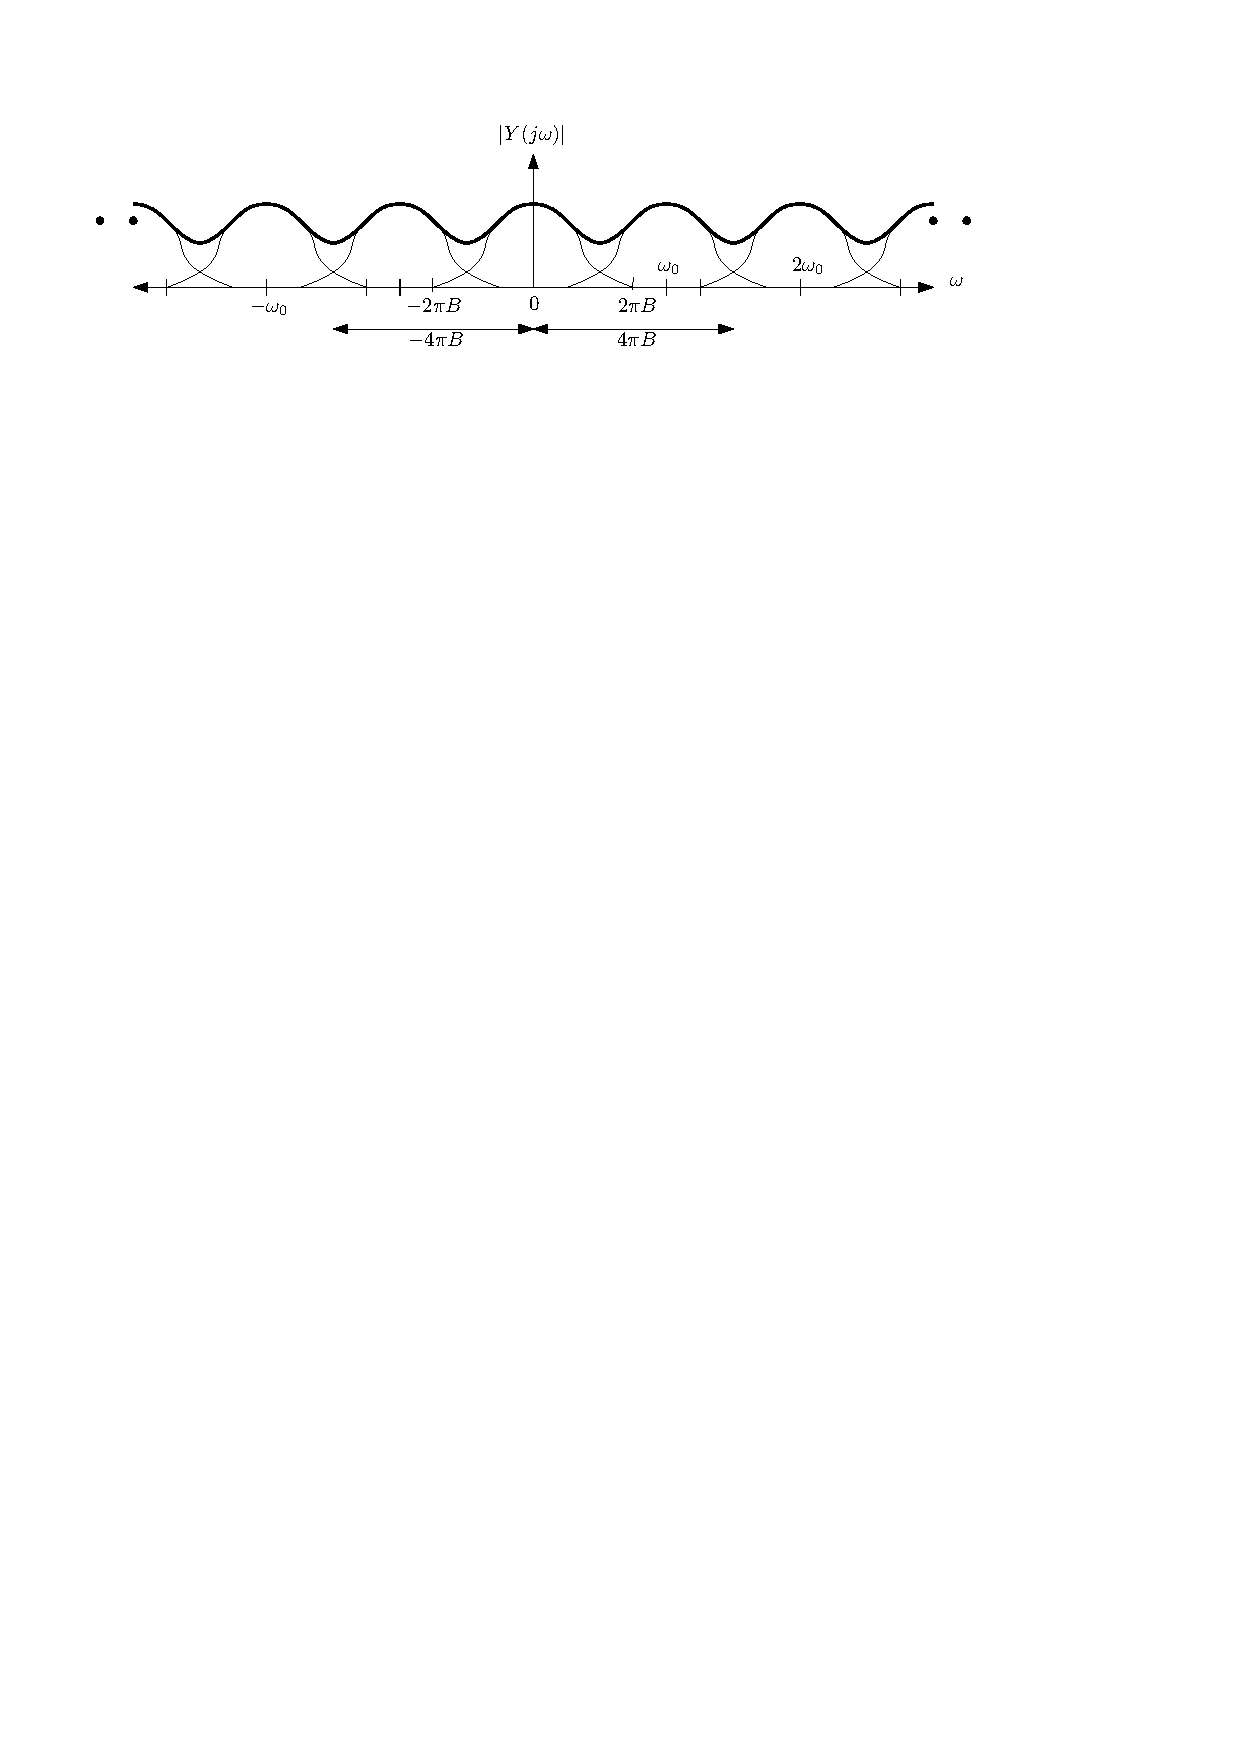
\includegraphics[scale=1]{graphics/bandlimitedsampled2.pdf}
\end{center}
As we will see next time, to reconstruct the signal $x_2[n]$ back to $x_2(t)$ we need to ensure that $\omega_0 > 4\pi B$ rad/s or equivalently $f_0 > 2 B$ Hz, which requires the sample time $T_0 < \tfrac{1}{2B}$ seconds. This is called the \emph{Nyquist} sample rate/frequency. 

\begin{example} Consider a signal representing a musical chord (an additive mixture of three notes)
  \[
  x(t) = \sin(2\pi\cdot (261) t) + \sin(2\pi\cdot (329) t) + \sin(2\pi\cdot (392) t) 
  \]
  Suppose it is sampled at a frequency of $f_0 = 1$ kHz. Then there is no aliasing into the frequency range $(0, 500)$ Hz. After reconstruction $x(t)$ would be unmodified. Suppose instead it is sampled at $f_0 = 500$ Hz. Then the signal component at $261$ Hz aliases to $239 = 500-261$ Hz, the signal component at $329$ Hz aliases to $171 = 500-329$ Hz, and the signal component at $392$ Hz aliases to $108 = 500-392$ Hz. When reconstructed, the signal now has an additional 3 tones mixed in at audible frequencies, but do not correspond to (Western) musical notes, i.e.
  \[
  x(t) = \sin(2\pi\cdot (108) t) + \sin(2\pi\cdot (171) t) + \sin(2\pi\cdot (239) t) + \sin(2\pi\cdot (261) t) + \sin(2\pi\cdot (329) t) + \sin(2\pi\cdot (392) t) 
  \]
\end{example}

\section{Practical Sampling}

Sampling in practice requires addressing three issues. First, we cannot generate the impulse train, but can only approximate it. Second, digital signals must have a fixed bit width so we have to convert the real signal value to a \emph{quantized} one. Lastly, since in general we have no control over the input signal means we need to ensure the signal is approximately band-limited before sampling.

\subsection{Sample and Hold}
Sampling is typically accomplished using a circuit called a \emph{sample-and-hold}, schematically illustrated below.

\begin{center}
  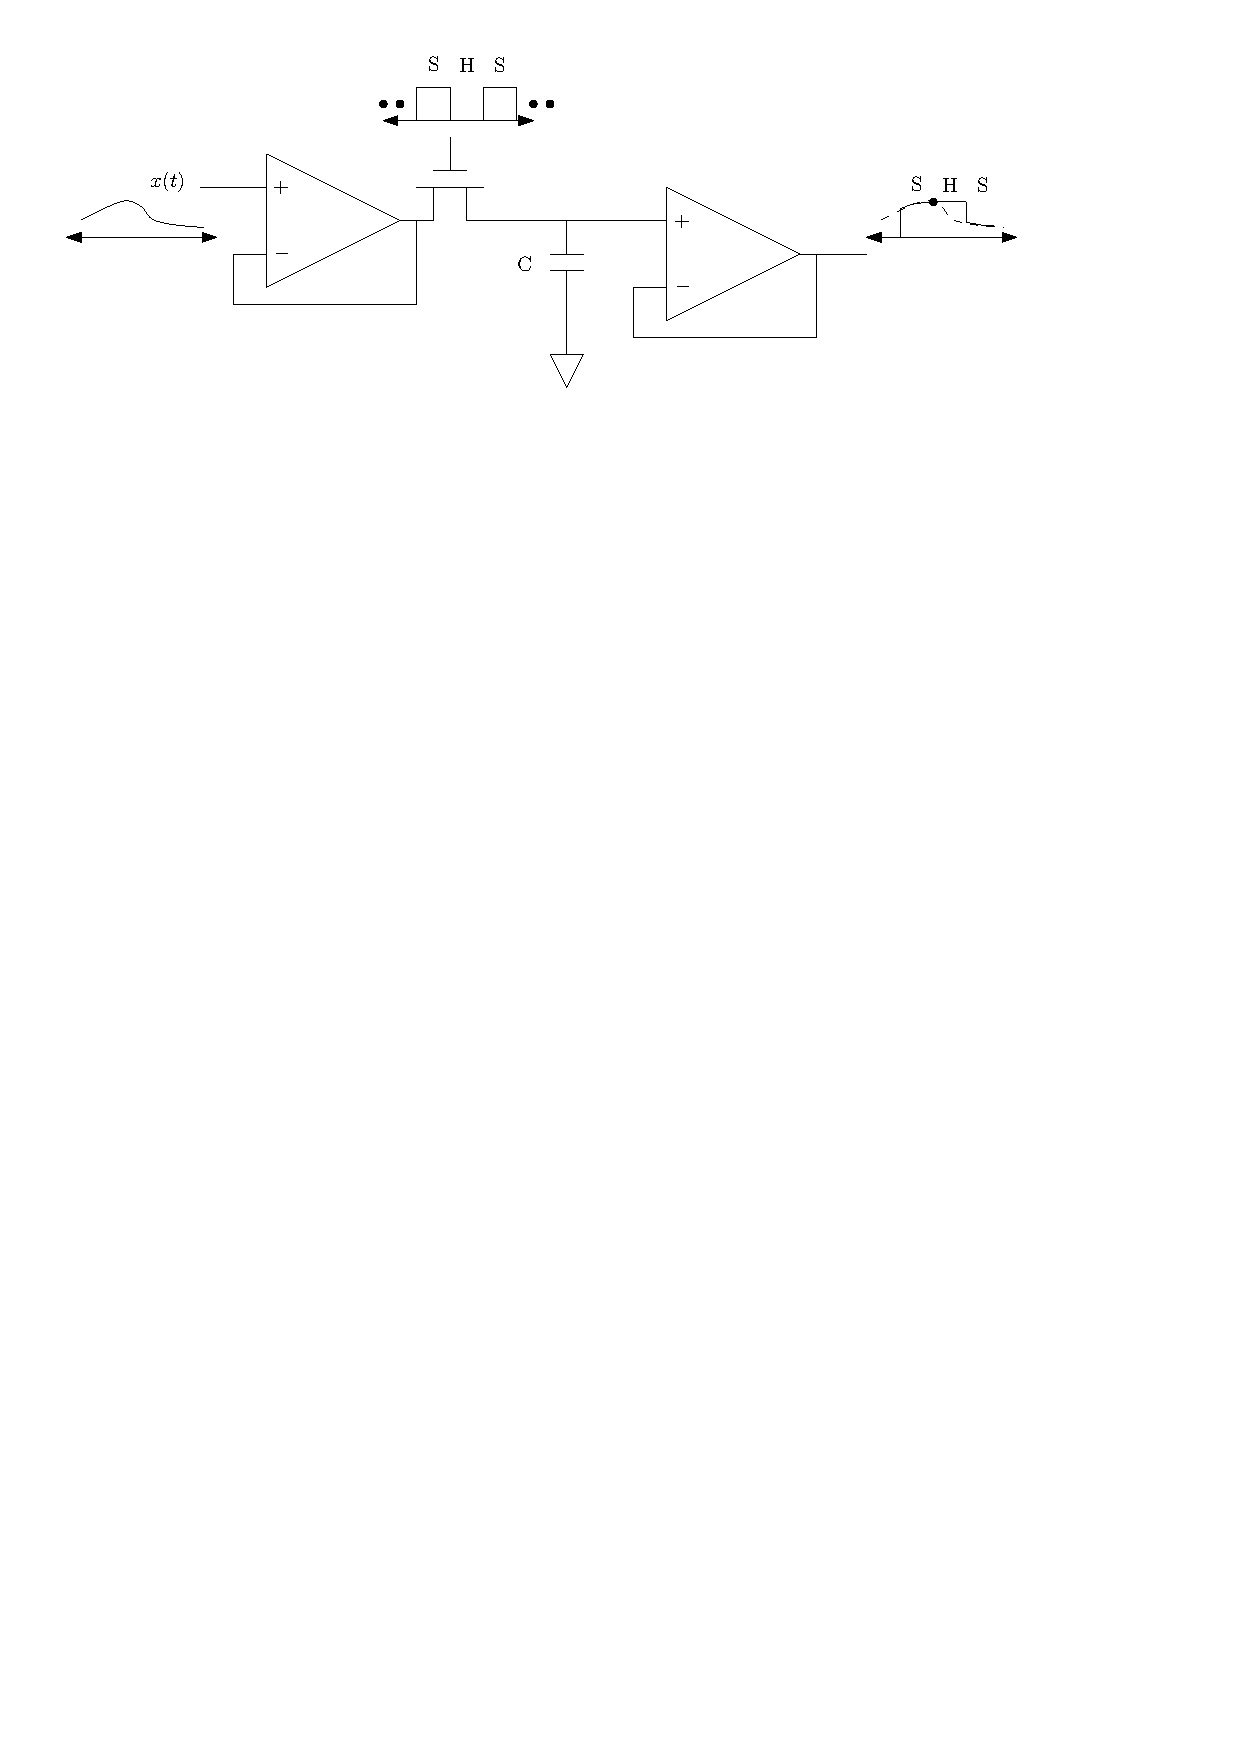
\includegraphics[scale=0.8]{graphics/smaple_hold.pdf}
\end{center}


The CT signal is applied to the input of the first op-amp buffer. The output of this first buffer is switched into a charging capacitor for the \emph{sample time}, then disconnected (high impedance) at regular intervals for the \emph{hold time}, typically using a MOSFET switch. The effect is the capacitor is charged to the current value of $x(t)$ during the sample-time, which it maintains during the hold-time, the value of which is bufered by the second op-amp. This can be mathematically modeled as a pulse train with a width equal to the sample time rather than as an impulse train.

\subsection{Quantization}

To quantize the signal after the sample-and-hold into $N$ bits, several strategies can be used. One popular approach is called \emph{successive approximation}, illustrated below

\begin{center}
  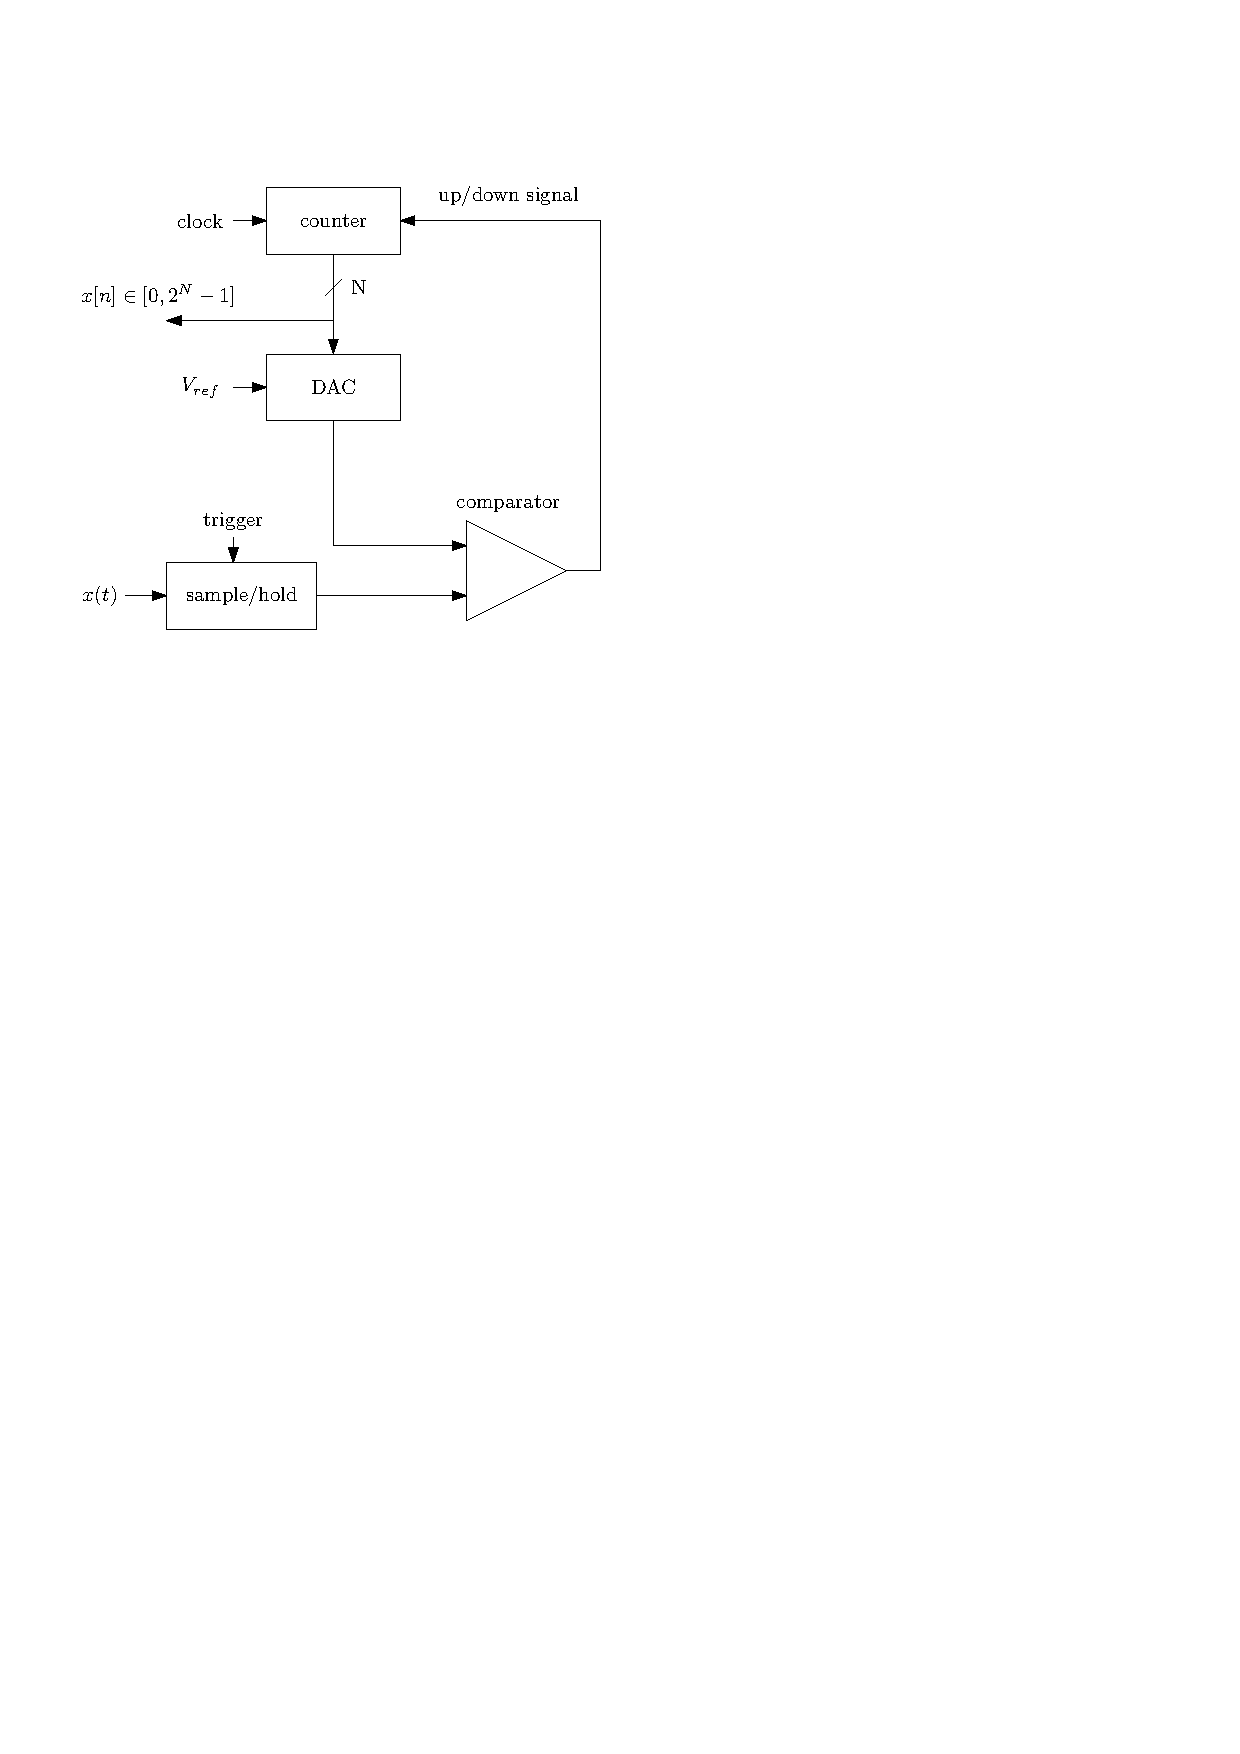
\includegraphics[scale=1]{graphics/sar.pdf}
\end{center}

The current quantized digital value is held in a counter connected to a clock signal. The direction of the counter (up or down) is controlled by a comparator connected to the output of the sample and hold and the current counter output and a digital-to-analog converter (DAC, usually a resistor ladder) that converts it back to an analog value. If the DAC value is less than the held value, the counter counts up, if the DAC value is greater than the held value the counter counts down. In this fashion the counter output tracks the held value after a settling time required for convergence, at which point the counter value is clocked into a register for storage.

\subsection{Anti-aliasing}

Before the sample and hold we need to include a filter to limit the bandwidth. This can be accomplished by a CT low-pass filter called an \emph{anti-aliasing} filter whose cutoff frequency in the ideal case is $\omega_c = 2\pi B$. As we saw in lecture 24 ideal filters cannot be implemented, thus we specify the anti-aliasing filter as a pass-band gain/frequency and a stop-band gain/frequency. Since the transition band is non-zero for a practical filter, this means we have to either lower the pass-band relative to the ideal or increase the sample rate. In the best case, the filter should have a stop-band frequency at half the sampling frequency with the order of the filter and pass-band frequency adjusted as needed. Alternatively the gain that defines the stop-band can be relaxed. This gives a desired frequency response magnitude that looks like the following.

\begin{center}
  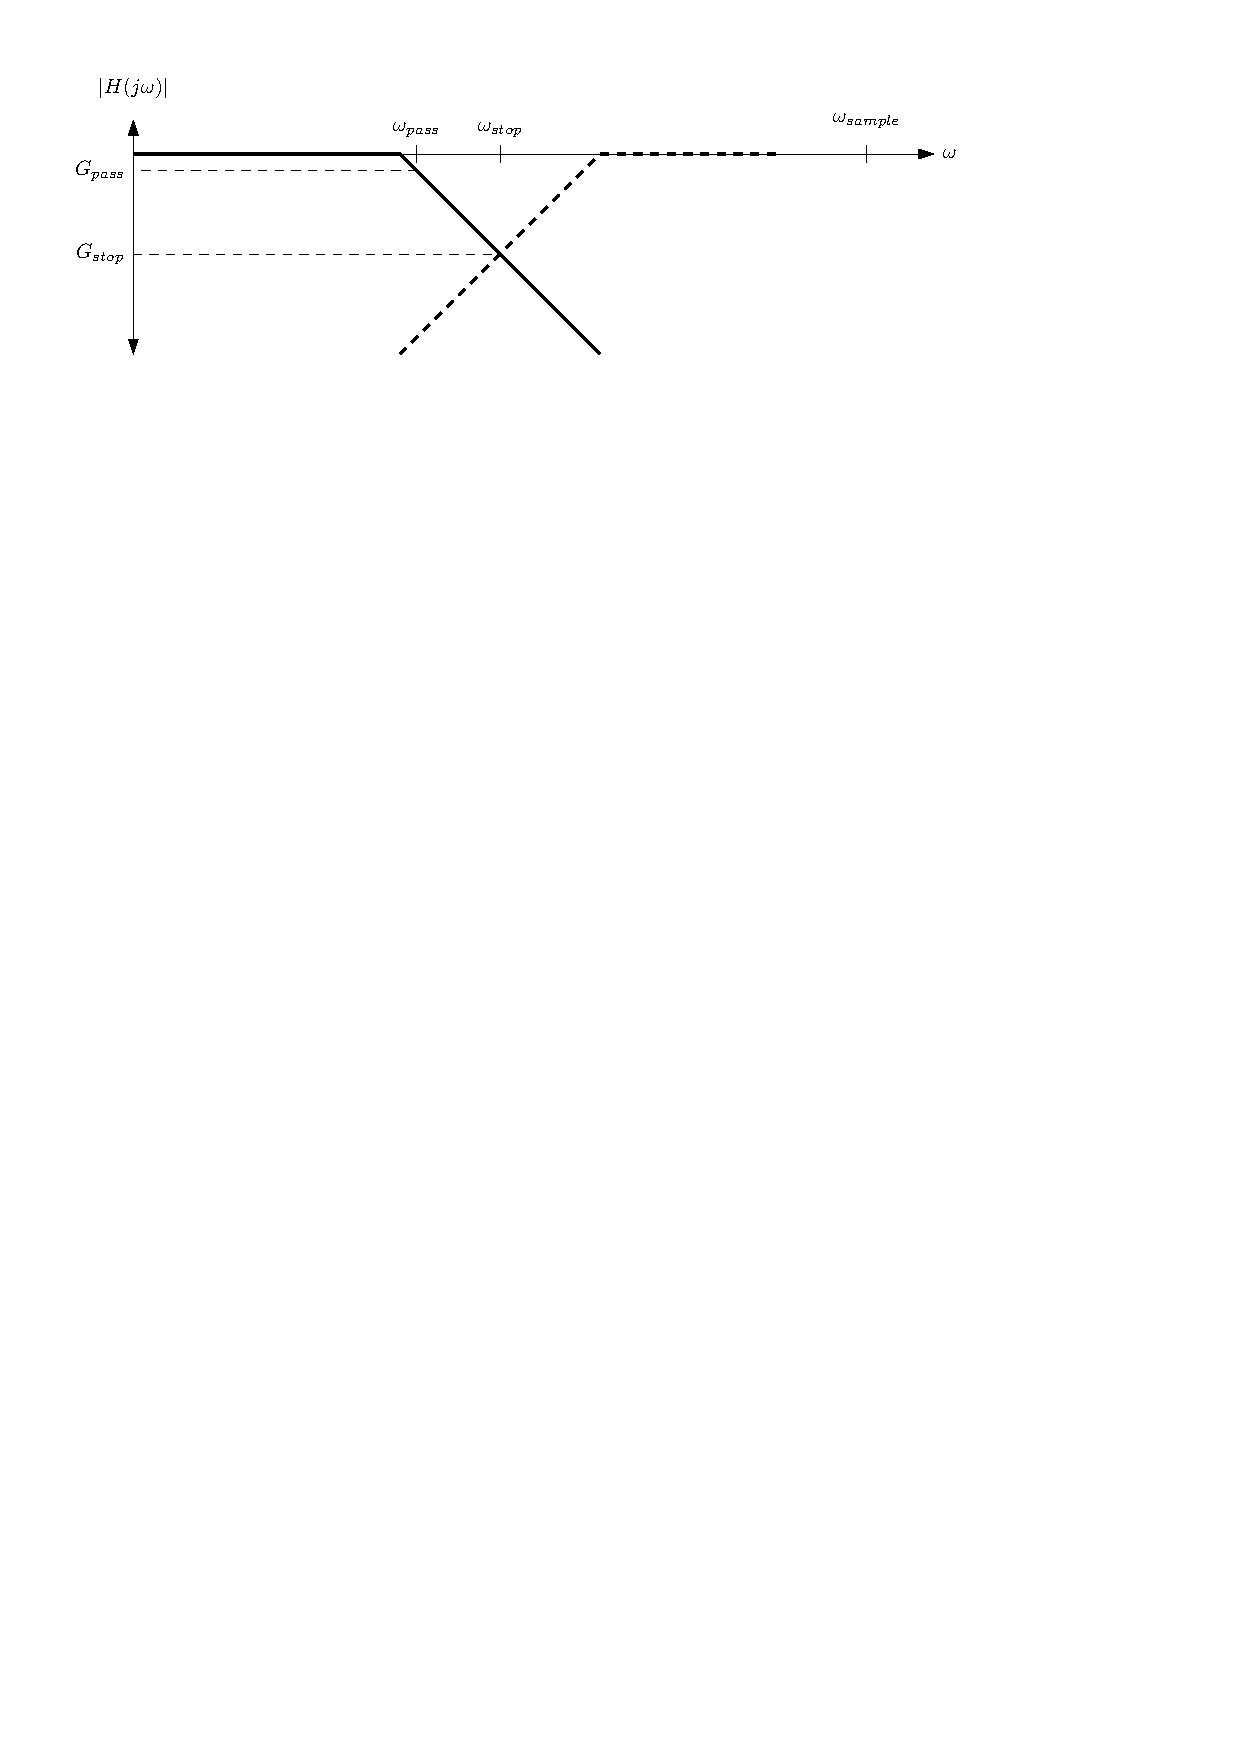
\includegraphics[scale=1]{graphics/antialias.pdf}
\end{center}
The bold dotted line shows the maximum frequency response of the first image.  
